\documentclass[11pt,letterpaper]{article}

% ── Packages ──────────────────────────────────────────────
\usepackage[margin=1in]{geometry}
\usepackage{amsmath,amssymb}
\usepackage{mathtools}
\usepackage{booktabs}
\usepackage{enumitem}
\usepackage{hyperref}
\usepackage[dvipsnames]{xcolor}
\usepackage{titlesec}
\usepackage{microtype}
\usepackage{parskip}
\usepackage{tikz}
\usetikzlibrary{arrows.meta,positioning,calc,fit}

% ── Formatting ────────────────────────────────────────────
\hypersetup{colorlinks=true, linkcolor=NavyBlue, citecolor=NavyBlue, urlcolor=NavyBlue, pdfstartview=FitH}
\titleformat{\section}{\large\bfseries}{\thesection}{1em}{}
\titleformat{\subsection}{\normalsize\bfseries}{\thesubsection}{1em}{}
\titleformat{\subsubsection}{\normalsize\itshape}{\thesubsubsection}{1em}{}

% ── Math shortcuts ────────────────────────────────────────
\newcommand{\bfp}{\mathbf{p}}
\newcommand{\bfz}{\mathbf{z}}
\newcommand{\bfy}{\mathbf{y}}
\newcommand{\bfd}{\mathbf{d}}
\newcommand{\cS}{\mathcal{S}}
\newcommand{\R}{\mathbb{R}}
\newcommand{\pp}{\,\text{pp}}

\begin{document}

% ── Title ─────────────────────────────────────────────────
\begin{center}
{\LARGE\bfseries Neural Field Perceiver}\\[6pt]
{\large Cross-Patient Speech Decoding from Intra-Operative $\mu$ECoG\\via Coordinate-Aware Encoding with Reprojection Supervision}\\[12pt]
{\normalsize Ben Tang \quad\textbar\quad Greg Cogan Lab, Duke University}\\[4pt]
{\normalsize April 2026 \quad\textbar\quad Version 11}
\end{center}

\medskip\noindent\rule{\textwidth}{0.4pt}\medskip

\noindent Technical design document for the Neural Field Perceiver.
Two new ideas: (1) coordinate-aware electrode encoding with learnable geometric calibration, (2) reprojection loss as spatial alignment supervision. Everything else is standard.
Claims are labeled \textbf{supported by related work}, \textbf{internally observed}, or \textbf{working hypothesis}.
Structural assumptions that could be wrong are marked in \textcolor{BrickRed}{red}.

\tableofcontents
\newpage


%% ====================================================================
%%  SECTION 1: PROBLEM
%% ====================================================================

\section{Problem}\label{sec:problem}

Each patient's $\mu$ECoG array is a sparse spatial sample of cortical activity during speech. The array sits on left ventral sensorimotor cortex (vSMC), and its position in MNI-152 space is determined post-hoc from electrode reconstruction (availability for our cohort is conditional --- see Section~\ref{sec:data}).

\textbf{Hardware.} Custom liquid crystal polymer thin-film (LCP-TF) arrays fabricated by Dyconex~\cite{duraivel2023}. Two configurations:

\begin{table}[ht!]\centering\small
\begin{tabular}{@{}lll@{}}
\toprule
& \textbf{128-channel (DBS)} & \textbf{256-channel (craniotomy)} \\
\midrule
Grid & $8 \times 16$ & $12 \times 22$ \\
Pitch & 1.33\,mm & 1.72\,mm \\
Footprint & ${\sim}11 \times 21$\,mm & ${\sim}21 \times 38$\,mm \\
Contacts & 200\,$\mu$m exposed diameter & 200\,$\mu$m exposed diameter \\
Placement & Through DBS burr hole & Directly on exposed cortex \\
\bottomrule
\end{tabular}
\end{table}

\noindent The LCP substrate is \textbf{physically flexible} --- the array conforms to the curved cortical surface during placement, so 3D electrode positions are non-planar even though the manufactured film is flat. Electrode reconstruction software (BioImage Suite / Brainlab) computes each electrode's individual MNI coordinate post-hoc, capturing this surface conformance. In-vivo impedance ranges 12.9--81.3\,k$\Omega$; electrodes $> 1$\,M$\Omega$ are excluded. Recording at 20\,kHz via Intan RHD2000 system; signal processed to HGA at 200\,Hz (see Section~\ref{sec:data}).

\textbf{Input.} For patient $i$ with $N_i$ electrodes at MNI positions $\{\bfp_j^{(i)}\}$, we observe high-gamma analytic amplitude (HGA, 70--150\,Hz) at 200\,Hz:
\begin{equation}\label{eq:observation}
d_j^{(i)}(t) = a\bigl(\bfp_j^{(i)},\; t\bigr) + \epsilon_j^{(i)}(t)
\end{equation}
where $a(\bfp, t)$ is the cortical HGA field and $\epsilon$ captures noise, impedance variation, and sub-electrode activity. Because the array is flexible, the MNI positions $\bfp_j^{(i)}$ are per-electrode 3D coordinates (not a rigid grid projection) --- the non-planar surface conformance is already captured.

\textbf{Output.} Infer the phoneme sequence $\bfy = (y_1, y_2, y_3)$ from a 9-phoneme vocabulary --- three separate 9-way classifications per non-word token (e.g., /a/, /b/, /e/).

\textbf{Cross-patient challenge.} Electrode $j$ on patient $i$ and electrode $j$ on patient $i'$ sample different cortical locations. Arrays are offset 15--25\,mm in MNI with variable rotation. Channel indices are meaningless across patients.

\begin{table}[ht!]
\centering\small
\begin{tabular}{@{}llr@{}}
\toprule
\textbf{Constraint} & \textbf{Value} & \textbf{Impact} \\
\midrule
Electrodes/patient & 63--201 sig.\ channels & Sparse cortical sampling \\
Electrode pitch & 1.33--1.72\,mm & Near-columnar resolution \\
Cross-patient offset & 15--25\,mm & Different cortical regions sampled \\
Trials/patient & 46--178 & Small-data regime \\
Utterance/patient & ${\sim}1$\,min & Too little for SSL \\
Phonemes & 9 classes $\times$ 3 positions & Low-dimensional output \\
\bottomrule
\end{tabular}
\end{table}


%% ====================================================================
%%  SECTION 2: KEY IDEA
%% ====================================================================

\section{Key Idea: Shared Neural Field + Reprojection}\label{sec:idea}

\subsection{Decomposition}

Cross-patient decoding requires shared structure. We model each patient's observations as:
\begin{equation}\label{eq:decomposition}
a^{(i)}(\bfp, t) = f(\bfp,\; t;\; \bfy) + r^{(i)}(\bfp, t)
\end{equation}
\begin{itemize}[leftmargin=2em]
\item $f$: shared neural manifold --- the low-dimensional surface that speech motor cortex activity evolves on during production, parameterized by articulatory state $\bfz(t) \in \R^k$ ($k {\approx} 5$--$8$; Section~\ref{sec:factorization}). Conserved across patients because somatotopic organization is conserved~\cite{safaie2023,gallego2020}; differently sampled because each patient's array sits at a different cortical location.
\item $r^{(i)}(\bfp, t)$: everything patient-specific, \textbf{varying per electrode}. Includes: per-electrode impedance differences (12.9--81.3\,k$\Omega$ range), spatial misalignment (${\sim}5$--$10$\,mm MNI error), differences in functional zone geometry (somatotopic \textit{ordering} is conserved, but the area, shape, and boundaries of each zone differ across patients), cortical folding, and pathology effects. Not a uniform scalar per patient --- $r^{(i)}$ is a spatially-varying field.
\end{itemize}
The architecture decomposes $r^{(i)}$ into components it can handle: rigid geometric correction ($\Delta, \omega$; 6 params) for the dominant spatial misalignment, and a patient embedding ($e^{(i)}$; 64 params) in the observation decoder. The decoder trunk $\phi(\tilde{\bfp}, e^{(i)})$ is a function of \textit{both} position and patient identity, so it learns spatially-varying patient effects: a noisy electrode at position $\bfp_j$ on patient $i$ gets a different $\phi$ than a clean electrode at the same MNI position on patient $i'$. This is how a single 64-dim embedding handles per-electrode variation without per-electrode parameters. Cross-patient decoding works to the extent that $\|f\| \gg \|r^{(i)}\|$.

\textbf{Preventing the residual from dominating.} Without explicit pressure, the model could dump information into patient-specific components and learn a trivial shared $f$. Three mechanisms prevent this: (1) \textbf{capacity bottleneck} --- $e^{(i)}$ is 64 dims entering only the decoder, and $\Delta/\omega$ is 6 scalars with L2 regularization; (2) \textbf{embedding dropout} --- during training, $e^{(i)}$ is set to $\mathbf{0}$ with probability $p_e = 0.5$, forcing the shared encoder and decoder trunk to carry the reconstruction signal without patient-specific shortcuts; (3) the encoder is architecturally patient-agnostic (no $e$), so $\mathcal{L}_{\text{class}}$ gradients flow entirely through the shared manifold. The embedding dropout is the critical mechanism: it directly trades off patient-specific vs.\ shared capacity, analogous to dropping skip connections to force information through the bottleneck.

\textbf{Anatomical grounding.} The shared field $f$ rests on somatotopic organization being cross-patient consistent. The literature provides quantitative constraints:

\begin{itemize}[leftmargin=2em]
\item \textbf{Gross somatotopic order (medial$\to$lateral) is conserved.} Roux et al.~\cite{roux2020} mapped 100 patients via direct electrostimulation to MNI space and found ``rare inter-individual variations'' in somatotopic ordering. Individual motor representations occupied $< 10$\,mm$^2$ areas. The ordering (leg $\to$ hand $\to$ face) is essentially invariant.
\item \textbf{Speech motor cortex has the highest positional variability (${\sim}$15--25\,mm).} The subcentral region shows five distinct sulcal morphological types~\cite{eichert2020}. Speech-related fMRI peaks in vSMC show SDs of ${\sim}8$--$12$\,mm per axis, meaning the full inter-individual spread is 20--25\,mm. Anatomical alignment reduces but does not eliminate this variability.
\item \textbf{Functional connectivity is the most conserved.} Primary sensorimotor areas sit at the low end of a sensory-fugal gradient where association cortex shows the highest inter-individual variability. Sensorimotor cortex has the most conserved wiring patterns~\cite{mueller2013}.
\end{itemize}

\textbf{Implication:} a shared spatial map \textit{exists} (conserved topology, conserved connectivity), but its absolute position varies by ${\sim}15$--$25$\,mm across patients. MNI normalization provides a rough frame ($\pm 5$--$10$\,mm error; see Section~\ref{sec:tokens}) within which the model must learn to localize the shared structure. The architecture must tolerate centimeter-scale positional uncertainty while exploiting the conserved somatotopic ordering.

\subsection{The factorization}\label{sec:factorization}

The shared field $f$ factorizes through a low-dimensional bottleneck:
\begin{equation}\label{eq:obs-function}
d_j^{(i)}(t) = g\bigl(\bfp_j^{(i)},\; \bfz(t)\bigr) + r^{(i)}\bigl(\bfp_j^{(i)},\; t\bigr) + \epsilon_j^{(i)}(t)
\end{equation}
where:
\begin{itemize}[leftmargin=2em]
\item $g(\bfp, \bfz)$: the \textbf{somatotopic map} --- given a brain position and an articulatory state, what is the neural activity? Time-invariant. Absorbs all spatial dependence.
\item $\bfz(t) \in \R^k$ ($k {\approx} 5$--$8$): the \textbf{articulatory state} --- tongue position, lip aperture, voicing, etc. Absorbs all time and phoneme dependence.
\end{itemize}

Space and time interact only through the $k$-dimensional bottleneck $\bfz(t)$. Instead of learning every (position $\times$ time $\times$ phoneme) combination, the model learns a spatial basis $g$ and temporal dynamics composed through $\bfz$.

\textcolor{BrickRed}{\textit{Aspirational, not enforced:}} The architecture's latent representation is $s(t) \in \R^{L \times d}$ ($L{=}16$, $d{=}64$, total 1024 dims per frame) --- vastly overcomplete relative to $k {\approx} 5$--$8$. The factorization is the low-parameter \textit{solution} we hope gradient descent finds, not a hard constraint the architecture enforces. The main inductive bias toward this factorization is that the spatial distance bias in attention is \textbf{static} (same spatial weighting at every time step), consistent with $g$ being time-invariant. But temporal self-attention can in principle learn time-varying spatial modulations through the values.

\textbf{The somatotopic map is static.} $g$ does not change during a trial. Cross-patient alignment is therefore a static geometric problem. The temporal dynamics $\bfz(t)$ are shared across patients --- the same phoneme produces similar trajectories regardless of who speaks it.


\subsection{The 3D vision analogy}\label{sec:analogy}

This structure maps to multi-view 3D reconstruction:

\begin{table}[ht!]\centering\small
\begin{tabular}{@{}ll@{}}
\toprule
\textbf{3D Reconstruction} & \textbf{Neural Field Decoding} \\
\midrule
3D body model & Shared somatotopic map $g(\bfp, \bfz)$ \\
Pose parameters & Articulatory state $\bfz(t)$ \\
Camera extrinsics (rough) & MNI positions (${\pm}5$--$10$\,mm error) \\
Bundle adjustment & Learned $\Delta^{(i)}, \omega^{(i)}$ \\
Camera intrinsics & Per-patient gain/bias ($e^{(i)}$) \\
2D keypoints & Electrode observations $d_j^{(i)}(t)$ \\
\textbf{Reprojection loss} $\|\pi(V) - x\|^2$ & \textbf{Reprojection loss} $\|g(\bfp, \hat{\bfz}) - d\|^2$ \\
\bottomrule
\end{tabular}
\end{table}

\textbf{MNI as rough extrinsics.} In multi-view reconstruction, initial camera poses are often noisy estimates refined by bundle adjustment. Similarly, intraoperative MNI coordinates carry ${\sim}5$--$10$\,mm total error (Section~\ref{sec:tokens}) --- good enough to establish the rough spatial frame, too imprecise for fine-grained spatial alignment. The learnable geometric correction ($\Delta, \omega$) serves as bundle adjustment, and the reprojection loss provides the gradient signal to drive it.

\textbf{Where the analogy breaks.} (1) Each patient is a different ``scene,'' not a different camera on the same scene --- the shared structure is weaker than photometric consistency. (2) We have 63--201 electrodes, not 65K pixels --- the reprojection signal per frame is thin. (3) The ``scene'' changes every frame. These mean reprojection is a useful regularizer, not the primary signal. The supervised classification loss remains primary.

\subsection{Evidence and central hypothesis}

\textbf{Central hypothesis.} \textit{Intra-operative $\mu$ECoG speech recordings share enough spatiotemporal structure across patients that a coordinate-aware spatial encoder, trained with reprojection supervision, will improve cross-patient phoneme decoding beyond methods that treat each patient's electrode array as unrelated.} This is testable via ablation A1 (Section~\ref{sec:ablations}).

\textbf{Supported by related work.}
Per-patient input layers + shared backbone transfers in adjacent settings: Singh~\cite{singh2025} ($N{=}25$ sEEG, PER 0.49 group vs.\ 0.57 individual); Willett~\cite{willett2023} (per-day affine + shared GRU).
Articulatory somatotopy in vSMC is reproducible~\cite{metzger2023,bouchard2013}.
MNI coordinates improve cross-patient ECoG transfer: Chen~\cite{chen2025} (SwinTW, PCC 0.765 on unseen patients).%
\footnote{Standard ECoG (10\,mm spacing), not $\mu$ECoG (2\,mm). None of these results use intra-operative recordings, $\mu$ECoG resolution, or our small-data regime.}

\textbf{Internally observed.}
LOPO achieves PER\,=\,0.762 on S14 (frozen backbone, grouped-by-token CV) --- above chance (0.89) but worse than per-patient (0.737).
55 experiments converge to PER 0.750--0.780, suggesting a systematic barrier not attributable to any single architectural choice.
Articulatory bottleneck head improves LOPO decoding, consistent with $f$ organized along articulatory dimensions.


%% ====================================================================
%%  SECTION 3: ARCHITECTURE
%% ====================================================================

\section{Architecture}\label{sec:architecture}

The encoder maps electrode observations and positions to a shared spatial representation:
\begin{equation}\label{eq:encoder}
s^{(i)}(t) = \text{Encoder}\bigl(\{d_j^{(i)}(t),\; \tilde{\bfp}_j^{(i)}\}_{j=1}^{N_i}\bigr) \in \R^{L \times d}
\end{equation}
with $L{=}16$ virtual electrodes and $\tilde{\bfp}_j^{(i)} = R(\omega^{(i)}) \cdot \bfp_j^{(i)} + \Delta^{(i)}$ the calibrated MNI position. The observation decoder predicts each electrode's activity:
\begin{equation}\label{eq:implemented}
\boxed{\hat{d}_j^{(i)}(t) = g_\theta\bigl(\tilde{\bfp}_j^{(i)},\; s_j^{*,(i)}(t),\; e^{(i)}\bigr)}
\end{equation}
where $s_j^{*,(i)}(t) = \sum_\ell a_{j\ell} \cdot s_\ell^{(i)}(t)$ is a position-weighted aggregation of virtual electrode outputs, and $e^{(i)}$ is a patient embedding.

\textbf{Patient identity split.} The encoder sees \textbf{no patient identity} --- only electrode positions and activity. The patient embedding $e^{(i)}$ enters only the observation decoder. The geometric correction ($\Delta, \omega$) adjusts positions but does not add non-geometric processing. This forces the latent $s^{(i)}(t)$ to represent the neural field in a patient-agnostic spatial frame.

\textcolor{BrickRed}{\textit{Position leakage:}} At $N{=}8$--$10$ training patients, each patient's unique electrode position set trivially identifies them --- the encoder can memorize patient-specific processing conditioned on geometry alone. The benefit of withholding $e$ is not preventing memorization during training but improving \textit{transfer to novel patients}: position-conditioned processing generalizes to new positions, while embedding-conditioned processing does not. Ablation A3 tests $e$ in encoder vs.\ decoder-only.


\subsection{Overview}\label{sec:overview}

\begin{center}
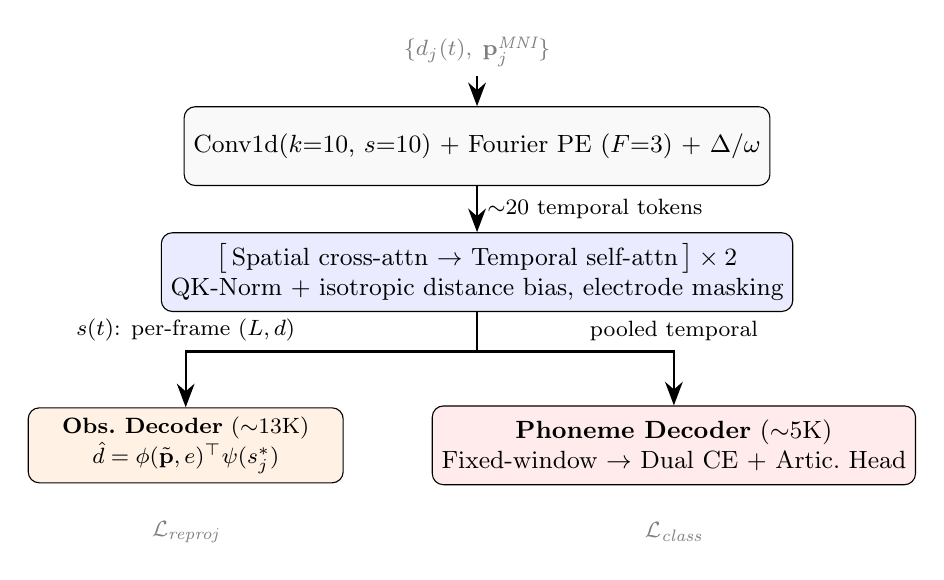
\begin{tikzpicture}[
  box/.style={draw, rounded corners, minimum width=5.5cm, minimum height=1cm, align=center, font=\small},
  smallbox/.style={draw, rounded corners, minimum width=4cm, minimum height=0.8cm, align=center, font=\footnotesize},
  arrow/.style={-{Stealth[length=3mm]}, thick},
  label/.style={font=\footnotesize\itshape, text=gray}
]

\node[box, fill=gray!5] (input) at (0, 0.8) {Conv1d($k{=}10$, $s{=}10$) + Fourier PE ($F{=}3$) + $\Delta/\omega$};

\node[box, fill=blue!8] (block) at (0, -0.8) {$\bigl[$\,Spatial cross-attn $\to$ Temporal self-attn\,$\bigr] \times 2$\\QK-Norm + isotropic distance bias, electrode masking};

\node[smallbox, fill=orange!10] (obs) at (-3.7, -3.0) {\textbf{Obs.\ Decoder} (${\sim}$13K)\\$\hat{d} = \phi(\tilde{\bfp}, e)^\top\psi(s_j^*)$};

\node[box, fill=red!8] (phoneme) at (2.5, -3.0) {\textbf{Phoneme Decoder} (${\sim}$5K)\\Fixed-window $\to$ Dual CE + Artic.\ Head};

\node[label] (raw) at (0, 2.0) {$\{d_j(t),\; \bfp_j^{\text{MNI}}\}$};

\draw[arrow] (raw) -- (input);
\draw[arrow] (input) -- (block) node[midway, right, font=\footnotesize] {${\sim}20$ temporal tokens};
\draw[arrow] (block.south) -- ++(0,-0.5) -| (obs.north) node[midway, above, font=\footnotesize] {$s(t)$: per-frame $(L,d)$};
\draw[arrow] (block.south) -- ++(0,-0.5) -| (phoneme.north) node[midway, above, font=\footnotesize] {pooled temporal};

\node[label] at (-3.7, -4.1) {$\mathcal{L}_{\text{reproj}}$};
\node[label] at (2.5, -4.1) {$\mathcal{L}_{\text{class}}$};

\end{tikzpicture}
\end{center}

\begin{equation}
\boxed{\mathcal{L} = \mathcal{L}_{\text{class}} + \lambda \,\mathcal{L}_{\text{reproj}}, \qquad \lambda = 0.3}
\end{equation}

Two losses, one weight, no annealing schedule. $\mathcal{L}_{\text{class}}$ drives phoneme decoding. $\mathcal{L}_{\text{reproj}}$ forces the encoder to build spatially meaningful representations that can predict physical observations --- the ``bundle adjustment'' signal. If reprojection competes with classification, set $\lambda{=}0$ (tested in A5).


\subsection{Electrode Tokens}\label{sec:tokens}

For electrode $j$ on patient $i$ at temporal bin $t'$:
\begin{equation}
\text{token}_j(t') = \underbrace{\text{Conv1d}(d_j; k{=}10, s{=}10)_{t'}}_{\text{temporal binning} \to d} + \underbrace{\text{Linear}\bigl(\gamma(\tilde{\bfp}_j) \to d\bigr)}_{\text{Fourier PE}} + \underbrace{\text{sin\_PE}(t')}_{\text{temporal position}}
\end{equation}

Three additive components: temporal content (electrode-specific, time-varying), spatial position (electrode-specific, constant), temporal position (shared).

\textbf{Temporal binning.} Per-electrode Conv1d($1 \to d$, $k{=}10$, $s{=}10$) on each electrode's HGA time series. Non-overlapping 50\,ms windows at 200\,Hz yield $T' = T/10 \approx 20$ tokens per electrode. Matches the field standard (Spalding, Willett: 20\,Hz effective rate). Shared across all electrodes and patients.

\textbf{Fourier positional encoding ($F{=}3$).} MNI coordinates are standardized so the speech motor region spans $[{-}1, 1]$ per axis ($1\,\text{unit} \approx 15$\,mm). Fourier features at three frequency levels:
\begin{equation}
\gamma(\bar{\bfp}) = \bigl[\sin(2^0 \pi \bar{\bfp}),\; \cos(2^0 \pi \bar{\bfp}),\; \ldots,\; \sin(2^{2} \pi \bar{\bfp}),\; \cos(2^{2} \pi \bar{\bfp})\bigr] \in \R^{18}
\end{equation}
Wavelengths: $\ell{=}0 \to 30$\,mm (full-array), $\ell{=}1 \to 15$\,mm (articulatory region), $\ell{=}2 \to 7.5$\,mm (sub-region). A linear projection $\text{Linear}(18 \to d)$ maps to token dimension.

\textbf{Why $F{=}3$, not higher.} Intraoperative MNI coordinates carry stacking errors:%
\footnote{Numbers from published surgical navigation and registration studies; specific values depend on imaging protocol, craniotomy size, and time since dural opening.}
\begin{itemize}[leftmargin=2em]
\item Neuronavigation registration: ${\sim}2$--$4$\,mm
\item Brain shift after craniotomy: ${\sim}2$--$10$\,mm (gravity-dependent, largest source)
\item MNI normalization (individual $\to$ template): ${\sim}2$--$3$\,mm (cortical surface)
\end{itemize}
Total uncertainty: ${\sim}5$--$10$\,mm RMS. The finest Fourier wavelength ($7.5$\,mm at $\ell{=}2$) sits just above this noise floor. $F{=}4$ ($3.75$\,mm) would encode spatial detail finer than MNI can resolve cross-patient, introducing noise rather than signal. Ablation A7 tests $F \in \{2, 3, 4\}$ and Linear PE (no Fourier).

\textbf{Learnable geometric calibration (per-patient, 6 params):}
\begin{itemize}[leftmargin=2em]
\item $\Delta^{(i)} \in \R^3$: translation (init $\mathbf{0}$). Absorbs systematic registration offset.
\item $\omega^{(i)} \in \R^3$: axis-angle rotation (init $\mathbf{0}$, Rodrigues formula). Absorbs orientation error.
\end{itemize}
These serve the same role as bundle adjustment in 3D reconstruction: the initial camera extrinsics (MNI coordinates) are refined during training to improve consistency across views (patients). The corrections apply to the \textbf{per-electrode MNI coordinates} (which already capture the flexible array's conformance to cortical curvature --- Section~\ref{sec:problem}), not to a rigid grid. What is approximately rigid is the \textit{registration error}: the neuronavigation system performs one registration per patient, and that systematic bias propagates uniformly to all electrode coordinates. Regularized with L2 ($10^{-3}$) and small init so they default to MNI when data is insufficient.

\textcolor{BrickRed}{\textit{Residual risk:}} Brain shift after craniotomy is non-rigid (gravitational deformation, ${\sim}2$--$10$\,mm), so rigid $\Delta/\omega$ captures only the dominant mode. The spatially smooth residual is absorbed by two mechanisms: (1) the soft Gaussian distance bias in attention degrades gracefully --- a few mm of position error still places each electrode in approximately the correct virtual electrode neighborhood; (2) the patient embedding $e^{(i)}$ in the decoder absorbs remaining patient-specific signal characteristics. Six scalars with L2 regularization provide a narrow information channel, limiting the risk of $\Delta/\omega$ serving as arbitrary patient codes.

The patient embedding $e^{(i)} \in \R^d$ (init ${\sim}\,\mathcal{N}(0, 0.02)$) enters only the observation decoder (Section~\ref{sec:obs-decoder}).


\subsection{Virtual Electrodes}\label{sec:virtual-electrodes}

$L = 16$ learned query vectors at learned MNI positions. Fixed model parameters, the same for every patient and time step. During spatial cross-attention, each virtual electrode attends to all real electrodes, weighted by spatial proximity and content.

After cross-attention, virtual electrode $\ell$ holds a $d$-dimensional summary of cortical activity near its position. The output $s(t) \in \R^{L \times d}$ is a spatially-indexed representation in a shared frame --- every patient maps to the same 16 positions regardless of electrode count or grid layout.

\textbf{Atlas initialization.} Positions initialized at Brainnetome atlas~\cite{fan2016} centroids of speech motor subregions (lip M1, tongue M1, jaw M1, laryngeal M1, lip S1, tongue S1, ventral premotor, SMA, etc.). This gives anatomically meaningful starting positions. Repulsive regularization prevents collapse. In practice, positions are unlikely to drift far from initialization --- the architecture is closer to ``atlas-anchored spatial ROIs with soft boundaries'' than ``learned cortical decomposition.''

\textbf{Why 16.} 63--201 electrodes cover ${\sim}20 \times 30$\,mm. 16 virtual electrodes gives ${\sim}5$\,mm spacing, roughly matching somatotopic scale. Ablation A4 tests $\{4, 8, 16, 32\}$.


\subsection{Spatiotemporal Blocks ($\times 2$)}\label{sec:blocks}

Each block alternates two attention operations:

\textbf{(a) Spatial cross-attention} (per temporal bin). Virtual electrodes (Q) attend to real electrode tokens (K, V). Attention logits use \textbf{QK-Norm} + \textbf{isotropic distance bias}:
\begin{equation}
A_{ij} = \tau_h \cdot \frac{Q_i \cdot K_j}{\|Q_i\|\,\|K_j\|} \;-\; \alpha_h \cdot \|\bar{\bfp}_i - \bar{\bfp}_j\|^2
\end{equation}
where $\tau_h > 0$ is a learnable temperature per head (init $\sqrt{d_h}$, clamped $\leq 100$), $\alpha_h > 0$ is a learnable distance scale per head (init $1.0$), $\bar{\bfp}$ denotes standardized MNI coordinates. QK-Norm (cosine similarity $\times$ temperature) keeps content and distance on comparable scales throughout training, following SwinV2~\cite{liu2022swinv2}. 4 heads, total 8 learnable scalars.

The distance bias is \textbf{static}: $\alpha_h$ depends only on head identity, not on time or input content. The spatial geometry of attention is the same at every time step, consistent with $g$ being time-invariant. What changes with time are the \textbf{values} (electrode activity), not the spatial weighting structure.

\textbf{(b) Temporal self-attention} (per virtual electrode). Each of 16 virtual electrodes attends across all ${\sim}20$ temporal tokens. 4 heads, sinusoidal temporal PE. Captures articulatory dynamics.

\textbf{Block internals.} Pre-LayerNorm residual connections. Standard ReLU FFN ($d_{\text{ff}} = 4d$). Dropout $p{=}0.2$ on attention weights and FFN output. DropPath $p{=}0.1$ on residual stream. Each block: LN $\to$ spatial cross-attn $\to$ LN $\to$ FFN $\to$ LN $\to$ temporal self-attn $\to$ LN $\to$ FFN.

\textbf{Electrode masking.} During training, mask 50\% of electrodes for all time steps (not included in KV set). The observation decoder still predicts at masked positions, forcing spatial interpolation from nearby unmasked electrodes. Fixed rate, no curriculum.%
\footnote{Tube masking (per-electrode temporal spans) would additionally force temporal interpolation, exercising both spatial and temporal structure. Extension ablation A10.}


\subsection{Why Perceiver, Not ViT or Point-Cloud Methods?}

\textbf{ViT} requires a fixed regular grid. Our patients have different grid sizes (8$\times$16, 12$\times$22) at different MNI positions. Cannot use.

\textbf{Point-cloud methods} (PointNet~\cite{qi2017}, Point Transformer~\cite{zhao2021}) handle irregular 3D point sets and are legitimate alternatives. Perceiver cross-attention is simpler for our case: shared query vectors directly provide the fixed-size shared output we need, and our 63--201 points are too small for hierarchical architectures. Worth testing as an ablation.


\subsection{Observation Decoder (${\sim}$13K params)}\label{sec:obs-decoder}

Predicts what each electrode should observe given the latent state. Structurally a DeepONet~\cite{lu2021}: branch encodes the latent field, trunk encodes spatial position and patient identity, interaction through low-rank inner product.

\textbf{Position-weighted aggregation.} Each electrode $j$ gets a local latent by weighting virtual electrode outputs by spatial proximity:
\begin{equation}
s_j^*(t) = \sum_{\ell=1}^{L} a_{j\ell} \cdot \text{out}_\ell(t), \qquad
a_{j\ell} = \frac{\exp\bigl(-\alpha_{\text{dec}} \cdot \|\bar{\tilde{\bfp}}_j - \bar{\text{v\_pos}}_\ell\|^2\bigr)}
             {\sum_{m} \exp\bigl(-\alpha_{\text{dec}} \cdot \|\bar{\tilde{\bfp}}_j - \bar{\text{v\_pos}}_m\|^2\bigr)}
\end{equation}

\textbf{Bilinear prediction.}
\begin{equation}\label{eq:bilinear}
\hat{d}_j^{(i)}(t) = \phi(\tilde{\bfp}_j,\; e^{(i)})^\top \;\psi\bigl(s_j^*(t)\bigr)
\end{equation}
$\phi = \text{MLP}(\tilde{\bfp}, e) \in \R^k$: spatial tuning (trunk). $\psi = \text{MLP}(s_j^*) \in \R^k$: latent activation (branch). $k{=}32$.

The decoder is the \textbf{only} component that sees patient identity. $\phi(\tilde{\bfp}, e)$ learns position-dependent patient effects (impedance, gain, tissue). During training, $e^{(i)}$ is dropped to $\mathbf{0}$ with probability $p_e{=}0.5$, forcing the trunk to learn position-dependent predictions that work \textit{without} patient identity --- the same regime used at zero-shot test time.

\textbf{Reprojection loss.}
\begin{equation}
\mathcal{L}_{\text{reproj}} = \frac{1}{N_i T} \sum_{t,j} \bigl\| d_j(t) - \hat{d}_j(t) \bigr\|^2
\end{equation}
Computed over all electrodes including masked ones (the model must spatially interpolate). This provides the ``bundle adjustment'' gradient: if $\Delta^{(i)}$ or $\omega^{(i)}$ is wrong, the reprojection at corrected positions will be worse, driving the geometric parameters toward better alignment.


\subsection{Phoneme Decoder (${\sim}$5K params)}\label{sec:phoneme-decoder}

\textbf{Spatial readout.} Mean-pool across $L$ virtual electrodes: $s_{\text{pool}}(t') = \frac{1}{L}\sum_{\ell} \text{out}_\ell(t')$. Yields $T' \approx 20$ temporal tokens.

\textbf{Fixed-window readout.} Divide the $T'$ temporal tokens into three equal windows (roughly corresponding to phoneme positions 1, 2, 3 in CVC/VCV tokens). Mean-pool each window:
\begin{equation}
\bfz_p = \frac{1}{|W_p|}\sum_{t' \in W_p} s_{\text{pool}}(t'), \qquad p \in \{1,2,3\}
\end{equation}

Dual head per position:
\begin{equation}
\text{logits}_p = \frac{1}{2}\bigl(\underbrace{\text{Linear}(\bfz_p \to 9)}_{\text{CE head}} + \underbrace{\tau \cdot \text{normalize}(\text{Linear}(\bfz_p \to 15)) \cdot A^\top}_{\text{articulatory head}}\bigr)
\end{equation}
$A \in \R^{9 \times 15}$: fixed articulatory feature matrix. $\tau$: learnable temperature. Separate heads per position.

$\mathcal{L}_{\text{class}} = \frac{1}{3}\sum_{p} \text{FocalCE}(\text{logits}_p, y_p;\; \gamma{=}2, \text{LS}{=}0.1)$ with mixup ($\alpha{=}0.2$).

Global readout $\bfz_{\text{global}} = \text{mean}(\text{all temporal tokens})$ for $k$-NN.


\subsection{Parameter Budget}

\begin{table}[ht!]\centering\small
\begin{tabular}{@{}lrll@{}}
\toprule
\textbf{Module} & \textbf{Params} & \textbf{Shared?} & \textbf{Role} \\
\midrule
Conv1d($1 \to 64$, $k{=}10$) & ${\sim}$0.7K & Shared & Temporal binning \\
Fourier PE + Linear($18 \to 64$) & ${\sim}$1.2K & Shared & Spatial encoding \\
Interleaved blocks ($\times 2$) & ${\sim}$200K & Shared & Spatial inversion + dynamics \\
\quad incl.\ isotropic $\alpha_h$ + $\tau_h$ & 8 & Shared & Distance scale + QK temp \\
\quad incl.\ virtual positions & 48 & Shared & Atlas-initialized MNI coords \\
Observation decoder & ${\sim}$13K & Shared & Reprojection forward model \\
Phoneme dual heads ($\times 3$) & ${\sim}$5K & Shared & Classification \\
\midrule
$\Delta^{(i)} + \omega^{(i)}$ & 6/pt & Per-patient & Geometric calibration \\
$e^{(i)}$ (decoder only) & 64/pt & Per-patient & Patient-specific reconstruction \\
\midrule
\textbf{Total shared} & $\mathbf{{\sim}220}$\textbf{K} & & \\
\textbf{Grand total} (10 pts) & $\mathbf{{\sim}221}$\textbf{K} & & (cf.\ current: 122K) \\
\bottomrule
\end{tabular}
\end{table}

The interleaved blocks dominate at ${\sim}200$K. A single block (${\sim}120$K total) is comparable to the current BiGRU baseline. Ablation A9 tests 1 vs.\ 2 blocks.

\textcolor{BrickRed}{\textit{Capacity concern:}} 220K params on ${\sim}1{,}300$ trials is aggressive. For classification alone ($3{,}900$ labels), this is ${\sim}56$ params per label. However, $\mathcal{L}_{\text{reproj}}$ provides additional supervision: $N_i \times T' \approx 100 \times 20 = 2{,}000$ data points per trial, so effective supervision is $2.6$M reconstruction targets $+$ $3.9$K classification labels. Electrode masking (50\%), dropout, and early stopping provide regularization. Whether this suffices is an empirical question.


%% ====================================================================
%%  SECTION 4: TRAINING AND EVALUATION
%% ====================================================================

\section{Training and Evaluation}\label{sec:training}

\subsection{Phase 1: Source training}

$N{-}1$ source patients. Each batch:
\begin{enumerate}[leftmargin=2em]
\item Construct tokens with Fourier PE at calibrated positions. Apply 50\% electrode masking.
\item Interleaved blocks: spatial cross-attn $\to$ temporal self-attn $\times 2$.
\item Reprojection on all electrodes including masked $\to \mathcal{L}_{\text{reproj}}$.
\item Fixed-window readout $\to$ dual head $\to \mathcal{L}_{\text{class}}$.
\item $\mathcal{L} = \mathcal{L}_{\text{class}} + \lambda \,\mathcal{L}_{\text{reproj}}$, $\lambda = 0.3$.
\end{enumerate}

AdamW with differential LR: shared params $10^{-3}$; geometric params ($\Delta, \omega$, virtual positions) $3 {\times} 10^{-4}$; patient $e$ at $10^{-3}$. Linear warmup (20 epochs) $\to$ cosine decay. Weight decay $10^{-4}$, grad clip 5.0, batch 16. Early stopping on held-out 20\% source validation, patience 7.

\subsection{Phase 2: Target adaptation (LP-FT)}

Per fold of 5-fold grouped-by-token CV on target patient:
\begin{enumerate}[leftmargin=2em]
\item \textbf{Linear probe.} Freeze encoder. Train decoder + $\Delta^{(\text{target})} + \omega^{(\text{target})} + e^{(\text{target})}$. 150 epochs. Best checkpoint.
\item \textbf{Fine-tune.} Unfreeze encoder at $0.1\times$ LR. 100 epochs, patience 7.
\end{enumerate}

\subsection{Evaluation regimes}

\begin{enumerate}[leftmargin=2em]
\item \textbf{Zero-shot.} Phase 1 only. $\Delta = \mathbf{0}$, $\omega = \mathbf{0}$, $e = \mathbf{0}$. No patient-specific params. Pure coordinates-only generalization. \textit{Note:} classification goes through the encoder + phoneme decoder (both patient-agnostic); the observation decoder is irrelevant at test time.
\item \textbf{LP-FT (primary).} Phase 1 $\to$ Phase 2. Matches clinical calibration scenario.
\end{enumerate}

\textbf{Metrics.} PER (edit distance), grouped-by-token 5-fold CV. Full recipe: weighted $k$-NN ($k{=}10$, cosine), TTA 16, dual head, source $k$-NN at $0.5\times$ weight.


%% ====================================================================
%%  SECTION 5: WHAT OUR EXPERIMENTS SHOW
%% ====================================================================

\section{What Our Experiments Show}\label{sec:experiments}

\subsection{Evaluation recipe matters more than architecture}

\begin{table}[ht!]
\centering\small
\begin{tabular}{@{}llrr@{}}
\toprule
\textbf{Component added} & \textbf{Category} & \textbf{PER} & \textbf{$\Delta$} \\
\midrule
Baseline (CE, mean-pool) & -- & 0.872 & -- \\
+ Label smoothing 0.1 & Training & 0.831 & $-4.1\pp$ \\
+ Per-position heads + dropout & Training & 0.819 & $-1.2\pp$ \\
+ Mixup $\alpha{=}0.2$ & Training & 0.802 & $-1.7\pp$ \\
+ Weighted $k$-NN ($k{=}10$) & Evaluation & 0.781 & $-2.1\pp$ \\
+ TTA (16 copies) & Evaluation & 0.767 & $-1.4\pp$ \\
+ Articulatory + CE dual head & Model & 0.737 & $-3.0\pp$ \\
\bottomrule
\end{tabular}
\end{table}

Cumulative marginal gains on S14, per-patient, grouped-by-token CV. Per-fold noise is $\pm 0.05$ PER.

\subsection{The ${\sim}0.76$ convergence}

55 LOPO experiments converge to PER 0.750--0.780. Root causes: (1) fixed CV fold structure --- fold 5 consistently ${\sim}$0.85, fold 4 ${\sim}$0.70; (2) ${\sim}$30 val samples/fold $\to$ $\pm 0.05$ noise; (3) S14 no longer truly held out (55+ architectures evaluated). Multi-scale temporal (stride 3+5+10) gave the largest single-change gain ($-1.6\pp$) but below the per-fold noise floor.

\subsection{SSL failed at this data scale}

All SSL methods near chance (PER 0.85--0.91) under grouped-by-token CV. With ${\sim}1$\,min utterance/patient, SSL cannot learn useful HGA representations.


%% ====================================================================
%%  SECTION 6: ABLATION PLAN
%% ====================================================================

\section{Ablation Plan}\label{sec:ablations}

\subsection{Core ablations (must run)}

\begin{table}[ht!]\centering\small
\begin{tabular}{@{}clp{6.5cm}@{}}
\toprule
\textbf{ID} & \textbf{Ablation} & \textbf{Question} \\
\midrule
A1 & Coordinate-aware encoding & \textbf{Central}: do coordinates help? \\
 & \quad a. Current Conv2d+BiGRU baseline & $\to$ 0.762 (anchor) \\
 & \quad b. Perceiver, no coordinate PE (uniform attn) & $\to$ architecture benefit alone \\
 & \quad c. Perceiver + Fourier PE & $\to$ coordinate benefit (c vs b) \\
 & \quad d. (c) + reprojection loss & $\to$ reprojection benefit (d vs c) \\
 & \quad e. (d) + $\Delta/\omega$ calibration & $\to$ calibration benefit (e vs d) \\
 & \quad f. (c) + random positions (sabotage) & $\to$ sanity check: MNI $>$ random \\
\midrule
A2 & Population-level (all patients) & Is the 0.76 wall S14-specific? \\
A3 & Patient identity split & $e$ in decoder-only vs.\ also in encoder \\
A4 & Virtual electrode count & $L \in \{4, 8, 16, 32\}$ \\
A5 & Reprojection weight & $\lambda \in \{0, 0.1, 0.3, 0.5\}$ \\
A6 & Cross-task data pooling & $+$ Duraivel 2025 data \\
A7 & Positional encoding variants & $F \in \{2, 3, 4\}$; Linear PE; no PE \\
\bottomrule
\end{tabular}
\end{table}

\subsection{Extension ablations (if core results are positive)}

\begin{table}[ht!]\centering\small
\begin{tabular}{@{}clp{6.5cm}@{}}
\toprule
\textbf{ID} & \textbf{Extension} & \textbf{Description} \\
\midrule
A8 & Anisotropic distance & Per-virtual-electrode $\Sigma_i$ (6 params each) \\
A9 & Block count & 1 block (${\sim}$120K) vs.\ 2 blocks (${\sim}$220K) \\
A10 & Tube masking & Electrode $\times$ time-window spans instead of full-electrode \\
A11 & Multi-scale temporal & Stride 3+5+10 (${\sim}126$ tokens) vs.\ stride 10 only \\
A12 & Learned position queries & Cross-attention readout vs.\ fixed windows \\
A13 & Cross-patient reproj.\ & Same-token $\mathcal{L}_{\text{cross}}$ with $e{=}\mathbf{0}$ \\
A14 & Bilinear vs.\ MLP decoder & $\phi^\top\psi$ vs.\ MLP$([\tilde{\bfp}; e; s_j^*])$ \\
\bottomrule
\end{tabular}
\end{table}


%% ====================================================================
%%  SECTION 7: PRIORITIES AND RISKS
%% ====================================================================

\section{Priorities and Risks}\label{sec:priorities}

\subsection{Priority ordering}

\begin{enumerate}[leftmargin=2em]
\item \textbf{Cross-task data pooling (A6).} Lowest risk. Same phonemes, overlapping patients~\cite{duraivel2025}. Directly addresses data scarcity. Works with current pipeline and new architecture.

\item \textbf{Population-level evaluation (A2).} Pure methodology fix. Required to distinguish S14-specific effects from universal trends. Must be the primary success criterion.

\item \textbf{MNI coordinate architecture (A1, this document).} Highest novelty, highest risk. The hypothesis that spatial alignment is the binding constraint is plausible but unvalidated.
\end{enumerate}

\subsection{Success criteria}

\textbf{Primary:} Mean PER across all patients improves over current LOPO baseline by $\geq 3\pp$ ($\geq 3$ seeds, LP-FT regime, paired Wilcoxon per-patient test at $\alpha{=}0.05$). MNI benefit isolated by A1c vs.\ A1b (coordinate value) and A1d vs.\ A1c (reprojection value).

\textbf{Interpretability:} Virtual electrode positions cluster over known speech motor regions (partially reflects atlas initialization --- stronger evidence would be positions that \textit{move away} from atlas priors coherently). Spatial tuning vectors $\phi(\bfp)$ recover articulatory somatotopy. Learned $\Delta^{(i)}$ are consistent with known registration quality.

\subsection{Risks}

\begin{table}[ht!]\centering\small
\begin{tabular}{@{}p{0.35\textwidth}cp{0.42\textwidth}@{}}
\toprule
\textbf{Risk} & \textbf{Severity} & \textbf{Mitigation} \\
\midrule
MNI coordinates unavailable & High & Fallback to scaled grid positions (A1b) \\
MNI precision too low ($>10$\,mm error) & High & $\Delta/\omega$ calibration; $F{=}2$ Fourier (A7) \\
Reprojection competes with classification & Med & $\lambda$ ablation A5; $\lambda{=}0$ fallback \\
220K params overfits 1{,}300 trials & Med & 1-block variant (A9); masking; early stop \\
Spatial alignment not the binding constraint & Med & If A1c $\approx$ A1b, coordinates don't help. A6 tests data scarcity alternative \\
Virtual electrodes collapse & Low & Atlas init; repulsive regularization \\
\bottomrule
\end{tabular}
\end{table}


%% ====================================================================
%%  SECTION 8: DATA
%% ====================================================================

\section{Available Data}\label{sec:data}

\begin{table}[ht!]\centering\small
\begin{tabular}{@{}lllcc@{}}
\toprule
\textbf{Cohort} & \textbf{Patients} & \textbf{Trials} & \textbf{MNI?} & \textbf{Usage} \\
\midrule
PS (Spalding published) & 8 patients$^\dagger$ & ${\sim}$1096 & Expected$^*$ & Source / target \\
PS (additional) & S16, S57$^\dagger$ & ${\sim}$250 & Expected$^*$ & Source \\
Cross-task (Duraivel 2025) & 3 overlapping pts & 156--208/pt & Expected$^*$ & Priority 1 \\
Lexical task & 13 patients & Varies & Expected$^*$ & Future source \\
\midrule
\textbf{Total unique PS} & \textbf{10 patients} & $\mathbf{{\sim}1350}$ & & \\
\bottomrule
\end{tabular}
\end{table}

\noindent $^\dagger$S32 = S36 (duplicate, counted once). 12 PS entries in BIDS $\to$ 11 unique $\to$ 10 usable (S18 excluded).

\noindent $^*$MNI coordinates available from BioImage Suite (DBS) / Brainlab (tumor) outputs on Box.%
\footnote{\textbf{Hard gate:} All MNI-dependent claims are conditional on extracting and auditing these coordinates. Fallback: scaled grid positions.}


% ── Bibliography ──────────────────────────────────────────
\begin{thebibliography}{99}\raggedright

\bibitem{singh2025}
Singh, A., et al.\ (2025).
Transfer learning via distributed brain recordings enables reliable speech decoding.
\textit{Nature Communications}, 16, 8749.

\bibitem{willett2023}
Willett, F.R., et al.\ (2023).
A high-performance speech neuroprosthesis.
\textit{Nature}, 620, 1031--1036.

\bibitem{metzger2023}
Metzger, S.L., et al.\ (2023).
A high-performance neuroprosthesis for speech decoding and avatar control.
\textit{Nature}, 620, 1037--1046.

\bibitem{bouchard2013}
Bouchard, K.E., et al.\ (2013).
Functional organization of human sensorimotor cortex for speech articulation.
\textit{Nature}, 495, 327--332.

\bibitem{chen2025}
Chen, J., et al.\ (2025).
Transformer-based neural speech decoding from surface and depth electrode signals.
\textit{Journal of Neural Engineering}, 22(1), 016017.

\bibitem{safaie2023}
Safaie, M., et al.\ (2023).
Preserved neural dynamics across animals performing similar behaviour.
\textit{Nature Neuroscience}, 26, 714--724.

\bibitem{gallego2020}
Gallego, J.A., et al.\ (2020).
Long-term stability of cortical population dynamics underlying consistent behavior.
\textit{Nature Neuroscience}, 23, 260--270.

\bibitem{spalding2025}
Spalding, Z., et al.\ (2025).
Shared latent representations of speech production for cross-patient speech decoding.
\textit{bioRxiv}. doi:10.1101/2025.08.21.671516

\bibitem{duraivel2023}
Duraivel, S., et al.\ (2023).
High-resolution neural recordings improve the accuracy of speech decoding.
\textit{Nature Communications}, 14, 6938.

\bibitem{duraivel2025}
Duraivel, S., et al.\ (2025).
Distinct neural processes link speech planning and execution.
\textit{bioRxiv}. doi:10.1101/2024.10.07.617122

\bibitem{roux2020}
Roux, F.-E., et al.\ (2020).
The human motor cortex somatotopy: from direct electrostimulation to functional MRI.
\textit{The Journal of Physiology}, 598(23), 5301--5316.

\bibitem{eichert2020}
Eichert, N., et al.\ (2020).
Morphological and functional variability in central and subcentral motor cortex of the human brain.
\textit{Brain Structure and Function}, 226, 263--279.

\bibitem{mueller2013}
Mueller, S., et al.\ (2013).
Individual variability in functional connectivity architecture of the human brain.
\textit{Neuron}, 77(3), 586--595.

\bibitem{liu2022swinv2}
Liu, Z., et al.\ (2022).
Swin Transformer V2: Scaling up capacity and resolution.
\textit{CVPR 2022}.

\bibitem{lu2021}
Lu, L., Jin, P., Pang, G., Zhang, Z., \& Karniadakis, G.E.\ (2021).
Learning nonlinear operators via DeepONet.
\textit{Nature Machine Intelligence}, 3, 218--229.

\bibitem{fan2016}
Fan, L., et al.\ (2016).
The Human Brainnetome Atlas: A new brain atlas based on connectional architecture.
\textit{Cerebral Cortex}, 26(8), 3508--3526.

\bibitem{qi2017}
Qi, C.R., et al.\ (2017).
PointNet: Deep learning on point sets for 3D classification and segmentation.
\textit{CVPR 2017}.

\bibitem{zhao2021}
Zhao, H., et al.\ (2021).
Point Transformer.
\textit{ICCV 2021}.

\bibitem{mildenhall2020}
Mildenhall, B., et al.\ (2020).
NeRF: Representing scenes as neural radiance fields for view synthesis.
\textit{ECCV 2020}.

\end{thebibliography}

\end{document}
